%%%%%%%%%%%%%%%%%%%%%%%%%%%%%%%%%%%%%%%%%%%%%%%%%%%%%%%%%%%%%%%%%%%%%%%%%%%%%%%%
%2345678901234567890123456789012345678901234567890123456789012345678901234567890
%        1         2         3         4         5         6         7         8
% DOCUMENT CLASS
\documentclass[a4paper,12pt]{Classes/RoboticsLaTeX}


% USEFUL PACKAGES
% Commonly-used packages are included by default.
% Refer to section "Book - Useful packages" in the class file "Classes/RoboticsLaTeX.cls" for the complete list.
\usepackage{amsmath}
\usepackage{amsfonts}
\usepackage{algorithm}
\usepackage{algorithmic}
\usepackage{multirow}
\usepackage{colortbl}
\usepackage{color}
\usepackage[table]{xcolor}
\usepackage{epigraph}
\usepackage{graphicx}
%\usepackage{subfigure}
\usepackage{caption}
\usepackage{acronym}
\usepackage{subcaption}
\usepackage{hyperref}
\usepackage{tabularx}
\usepackage{url}
%\usepackage{glossaries}
\usepackage{float}
\usepackage{longtable}
\usepackage[pdftex]{graphicx}
\usepackage{pdfpages}
\usepackage{pdflscape}
\usepackage[acronym,toc]{glossaries}
\usepackage{setspace}
\usepackage[utf8]{inputenc}
\usepackage[table]{xcolor}


%\usepackage{layout}

\setstretch{1.5}
%\onehalfspacing


% SPECIAL COMMANDS
% correct bad hyphenation
\hyphenation{op-tical net-works semi-conduc-tor}
\hyphenation{par-ti-cu-lar mo-du-le ge-stu-re}
% INTERLINEA 1.5
%\renewcommand{\baselinestretch}{1.5}

%% ignore slightly overfull and underfull boxes
%\hbadness=10000
%\hfuzz=50pt
% declare commonly used operators
%\DeclareMathOperator*{\argmax}{argmax}

% >>>> Replace all the [[Placeholders]] on the front page and in the Declaration <<<<

\title{\Large{Uncovering Optimal Solar Site
Locations using Autoencoder and Clustering with Application in India}}

\author{Smitesh Nitin Patil}
\collegeordept{School of Computer Science}
\university{University of Galway}
\crest{
\includegraphics[width=140mm]{Figures/University_Of_Galway_Logo__Positive_Landscape.png}}
%\crest{
\includegraphics[width=80mm]{Figures/University_of_Galway_logo_2022.png}}

\supervisor{Dr.Karl Mason}
%\supervisor{Name of the Supervisor}
%\supervisor{Name of the Co-Supervisor}	

% replace NAME with your name and PROGRAMME with Data Analytics, Artificial Intelligence, or Artificial Intelligence - Online
\degree{MSc in Computer Science (Data Analytics)}
\degreedate{[[Date of submission]]}  % Replace with submission date


%%%%%%%%%%%%%%%%%%%%%%%%%%%%%%%%%%%%%%%%%%%%%%%%%%%%%%%%%%%%%%%%%%%%%%%%%%%%%%%%
%%% uncomment if glossary needed, see examples in file
%\makeglossaries
%\loadglsentries{glossary}

\begin{document}


	\begin{spacing}{1}
		\maketitle
	\end{spacing}
	
	% add an empty page after title page
	%\newpage\null\thispagestyle{empty}\newpage
	
	% set the number of sectioning levels that get number and appear in the contents
	\setcounter{secnumdepth}{3}
	\setcounter{tocdepth}{3}
	
	\frontmatter
	
	% Replace NAME and THESIS-TITLE with your name and the title of this thesis.
	\textbf{DECLARATION} 
	I, Smitesh Nitin Patil, hereby declare that this thesis, titled ``Uncovering Optimal Solar Site
	Locations using Autoencoder and Clustering with applications in India'', and the work presented in it are entirely my own except where explicitly stated otherwise in the text, and that this work has not been previously submitted, in part or whole, to any university or institution for any degree, diploma, or other qualification. 
	\newline
	
	\begin{tabular}{@{}p{.5in}p{4in}@{}}
		Signature: & ~~\hrulefill \\
	\end{tabular}
	
	
	%%%% uncomment if acknowledgements needed
	%\textbf{Acknowledgement}
	%
	%
	%\newpage\textbf{}
	
	
	% THESIS ABSTRACT
	\begin{abstracts}
		This project delves into the integration of Autoencoders and clustering techniques within the framework of GIS (Geographical Information System) 
		data to pinpoint optimal locations for Solar PV (Photo-Voltaic) installations. By harnessing advanced machine learning methodologies in tandem with 
		spatial analysis, this research aims to carve out a novel approach, distinct from studies previously undertaken in this field, to the best of the authors' 
		knowledge. Through the analysis of diverse environmental, climatic, and topographical factors, the proposed methodology furnishes a holistic solution for 
		discerning areas with peak solar energy potential. The outcomes not only underscore the efficacy and robustness of the suggested approach but also highlight 
		its prospective applications in the wider scope of renewable energy planning.
		
		\textbf{Keywords: } Geospatial Information, Unsupervised Learning, Self-supervised
		Learning, Analytical-Hierarchical Process, Renewable energy, Site Selection,
		Spatial Analysis, Sustainability.
	\end{abstracts}
	
	
	\tableofcontents
	\listoffigures
	\listoftables

	\section*{Acronyms}
	\begin{acronym}
		\acro{MLP}{Multi-Layer Perceptron}
		\acro{MCDMs}{Multi-Criteria Decision-Making Methods}
		\acro{AHP}{Analytical Hierarchy Process}
		\acro{NREL}{National Renewable Energy Laboratory}
		\acro{SRTM}{Shuttle Radar Topography Mission} 
		\acro{DEM}{Digital Elevation Model}
		\acro{USGS}{United States Geological Survey}
		\acro{OSM}{OpenStreeMap}
		\acro{DNI}{Direct Normal Irradiance}
		\acro{GHI}{Global Horizontal Irradiance}
		\acro{DHI}{Direct Horizontal Irradiance}
		\acro{NSRDB}{National Solar Irradiance Database}
		\acro{CR}{Consistency Ratio}
		\acro{CI}{Consistency Index}
		\acro{RI}{Random Consistency Index}
		\acro{SOM}{Self-Organizing Map}
		\acro{BMU}{Best Matching Unit}
		\acro{PV}{Photo-Voltaic}
		\acro{NASA}{National Aeronautical and Space Agency}
		\acro{GIS}{Global Information System}
		\acro{PCA}{Principle Component Analysis}
		\acro{RBMs}{Restricted Boltzmann machines}
		\acro{CNN}{Convolutional Neural Network}
		\acro{CNNs}{Convolutional Neural Networks}
	\end{acronym}



	\printglossary[title=List of Acronyms,type=\acronymtype]

	
	
	\mainmatter
	
	
	\chapter{Introduction}
	\label{chap:introduction}

	\section{Motivation}
	

	The global transition from fossil fuel-based energy sources to sustainable alternatives like wind and solar is paramount for the 21st century. 
	The incentives for deploying these renewable sources are considerable. These resources are natural, free, abundant, and replenishable. Solar energy, 
	generated from photovoltaic cells, requires consistent high solar irradiance throughout the year to be profitable. Tropical regions, like parts of India, 
	benefit from abundant sunlight year-round.

	India's energy demands are escalating. It stands as the third-largest producer of electricity globally, following the United States and China\cite{bp2021}. 
	Presently, India's energy sector leans heavily on fossil fuels, with sources like coal fulfilling three-quarters of the country's energy needs. Nevertheless, 
	India is making significant investments in solar and hydropower projects. The nation's committed to ensuring renewable energy sources account for 
	50\% of energy consumption by 2030 and aspires to achieve net zero by 2070, as declared during the COP26 summit in 2021\cite{bbc2023}. This commitment 
	is evident as, between 2017 and 2021, India's solar power production capacity tripled, placing it third in global solar capacity rankings\cite{reuters2022}.

	Given the task's significance, it's crucial to rapidly identify new locations for renewable energy generation plants. The Indian government's national energy policy 
	prioritizes solar and hydroelectric power generation. Situated between latitudes 20.5937° N and 78.9629° E, India's temperate and tropical climate conditions ensure 
	high solar irradiance levels.

	Before pinpointing promising regions for solar farms, several factors require careful consideration: the slope gradient of the terrain, proximity to urban centers, and the 
	presence of conservation areas. Historically, scientific studies focusing on solar \ac{PV} plant installations, which leverage GIS data, have leaned towards the use of 
	\ac{MCDMs} to evaluate these factors\cite{reuters2022,colak2020,garni2017,zoghi2017,saraswat2021}. These studies predominantly employed the \ac{AHP} as their chosen \ac{MCDMs} 
	technique to determine the relevant criteria. This research, however, ventures into exploring novel unsupervised learning methods. These methods draw parallels with techniques \
	employed by researchers like Chang et al., who used them for monitoring landslide susceptibility using geospatial data\cite{chang2020}. Specifically, this study emphasizes the 
	use of Autoencoders and clustering techniques to pinpoint regions that hold importance for the establishment of solar \ac{PV} plants.

	Although similar research has been conducted in India, many of these studies faced constraints due to the limited resolution of spatial 
	data\cite{jain2011,saraswat2021,sindhu2017}. They also primarily relied on \ac{MCDMs} for classification. The data underpinning this study is sourced from a diverse array of 
	institutions, including the \ac{NREL} for solar irradiance, the \ac{DEM} provided by the \ac{SRTM} spearheaded by the \ac{USGS}, and \ac{OSM}. The latter offers detailed insights into land use, protected reserves, water bodies, 
	urban centers, and transportation networks.

	
	\section{Purpose}

	The primary objectives of this study are:

	\begin{enumerate}
		\item To develop an innovative approach utilizing unsupervised and self-supervised learning methodologies for pinpointing optimal geolocations for the establishment of solar PV plants.
		
		\item While prior studies on solar PV site selection in India were conducted with a limited scope, often relying on data with low spatial resolution (greater than 1000 meters), this research aims to leverage datasets with superior spatial resolution (ranging from less than 10 meters to 30 meters).
		
		\item To the student's best knowledge, no previous studies have employed self-supervised Autoencoder and clustering based classification for \ac{PV} sites on such a comprehensive scale.
	\end{enumerate}

	\section{Research Questions}

	\begin{enumerate}
		\item Given the vast and varied sources of data (e.g., \ac{NREL}, \ac{DEM} from \ac{SRTM}, \ac{OSM}), how can they be effectively integrated to yield the most comprehensive insights for solar site selection?
		\item Is it feasible to employ a novel technique that combines autoencoders and clustering to identify optimal areas for solar PV plant installations, based on data derived from the aforementioned sources?
	\end{enumerate}

	\chapter{Background and Related Work}

	This chapter highlights the methods used by researchers previous in the domain in form of a literature review.
	
	\section{Criteria and Factors Affecting Decision-making}

	Selecting the right features for predictive models is a pivotal step in making informed decisions about the feasibility of specific geolocations for solar \ac{PV} plants. There have been numerous studies undertaken by researchers to determine the critical factors for classifying \ac{PV} solar plant sites.

	Colak et al.\ conducted a study to identify suitable locations for establishing photovoltaic power plants in the Malatya province of Turkey\cite{colak2020}. The authors employed 11 layers of GIS data to pinpoint the most favorable sites. These layers encapsulated various factors that influence the decision-making process, such as:

	\begin{enumerate}
		\item \textbf{Solar Energy Potential:} Gauging the solar potential of a region is paramount. This metric essentially dictates the energy yield of a region when equipped with a photovoltaic power plant.
		
		\item \textbf{Slope:} The terrain's slope plays a crucial role in the decision-making process. A more level terrain is preferred for the installation of \ac{PV} panels, ensuring optimal exposure and ease of maintenance.
		
		\item \textbf{Transformer Centers and Energy Transmission:} Transmitting electricity over vast distances without the appropriate energy infrastructure results in significant energy losses. Hence, having a power transmission system in place is crucial when considering a location for a new plant.
		
		\item \textbf{Land Cover:} Certain lands designated as nature reserves, tribal habitats, or for other specific purposes are legally off-limits for energy generation activities. It's imperative to factor in these designations when choosing a site.
		
		\item \textbf{Residential Areas:} Constructing a solar plant near an urban center might pose future challenges, especially with the continuous expansion of urban sprawl. Conversely, having a \ac{PV} solar plant in proximity to urban centers can mitigate transmission losses. This duality necessitates a balanced consideration.
	\end{enumerate}

	For data preprocessing, various hardset conditions were set to restrict certain areas like slope elevation of land cannot be more than 20 percent,
	distance to road, rail network should be more than 0.1 km, no residential areas nearby and proximity to energy transmission network.

	\begin{figure}[H]
		\centering
		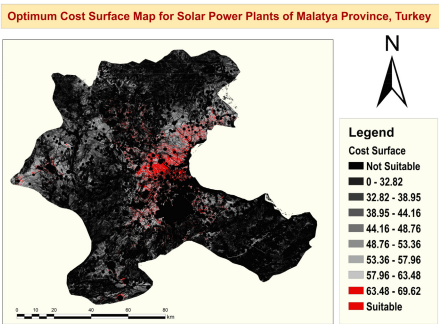
\includegraphics[width=0.5\textwidth]{Figures/Colak.png} % Adjust the width as needed
		\caption{Suitable sites for Solar Powerplant wiht cost factor by author Colak et al.\cite{colak2020}}
		\label{fig:my_label} % Use this label to reference the figure elsewhere
	\end{figure}

	A similar study was conducted by Al Garni et al. in Saudi Arabia\cite{garni2017}. The available land was categorized into five classes: least suitable, marginally suitable, 
	moderately suitable, highly suitable, and most suitable. The decision-making process for site selection unfolded in three phases:
	\begin{enumerate}
		\item Setting decision criteria and restrictions for the site selection study.
		\item Prioritizing sites with high solar potential.
		\item Conducting an analysis on the prioritized regions for informed decision-making.
	\end{enumerate}

	Like the aforementioned study, the authors relied on GIS data provided by NREL, selecting attributes that determined the criteria for site selection. 
	These included DEM, Solar irradiation, and Air Temperature. Broadly, these factors can be divided into two categories: technical (factors affecting energy production) 
	and economical (factors influencing the economic viability of the project).

	Zoghi et al. proposed dividing the factors into four major categories for their case study carried out in Isfahan province, Iran\cite{zoghi2017}:
	\begin{enumerate}
		\item \textbf{Environmental:} Land use, Protected Areas, Wetlands, and Water Resource.
		\item \textbf{Geomorphological:} Elevation, Slope, and Aspect.
		\item \textbf{Location:} Distance to City, Distance to Power line, and Distance to Transport network.
		\item \textbf{Climatic:} Sunshine, Cloudy Days, Dusty Days, Solar Radiation, Rainy and Snowy Days, and Humidity.
	\end{enumerate}

	The study carried out by Saraswat et al. (2021) represents the most elaborate case study for site selection of solar \ac{PV} plants in India, 
	to the best of the student's knowledge\cite{saraswat2021}. A significant limitation of this study is the data's spatial resolution. With a resolution of 
	around 1000m, it is not well-suited for detailed DEM modeling and other attributes. Consequently, the solar farm suitability map produced in this study lacks
	 granularity at a spatial level. However, various databases, provided by USGS and \ac{NREL}, offer spatial resolutions of 30m and can be employed to yield more accurate predictions.

	Data for the study were sourced from multiple governmental bodies: \ac{NREL} for solar radiation, DIVA-GIS for roads and inland water bodies, and the DEM model was provided by the United States Geological Survey (USGS). The factors were segmented into three categories: technical, socio-environmental, and economic.
	\begin{enumerate}
		\item \textbf{Technical:} Solar Radiation, Slope, Aspect, and Elevation.
		\item \textbf{Socio-Environmental:} Distance from coastline, Distance from water bodies, airports, and Land use.
		\item \textbf{Economic:} Distance from urban areas, roads, transmission lines, and power plants.
	\end{enumerate}

	\begin{figure}[H]
		\centering
		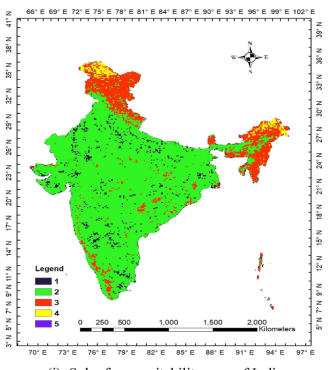
\includegraphics[width=0.5\textwidth]{Figures/Saraswat.png} % Adjust the width as needed
		\caption{ Optimal sites by level of importance by author \cite{saraswat2021}}
		\label{fig:my_label} % Use this label to reference the figure elsewhere
	\end{figure}
	

	\section{Analytical Hierarchical Process}

	\ac{MCDMs} have been extensively employed in literature for identifying optimal solar PV plant sites. 
	Unlike machine learning techniques, which automatically learn biases without being explicitly programmed, \ac{MCDMs} primarily focus on decision-making based on predefined criteria. 
	These criteria are often ranked manually to guide decision-making processes.

	\ac{AHP} is a widely recognized \ac{MCDMs} technique, as attested by numerous literary sources\cite{colak2020,saraswat2021,garni2017,zoghi2017}. 
	\ac{AHP} was pioneered by Prof. Thomas Saaty\cite{saaty1988}. At its core, \ac{AHP} emphasizes ranking criteria that influence the decision-making process. 

	The methodology of \ac{AHP} can be distilled into three stages:

	\begin{enumerate}
		\item \textbf{Problem Definition and Hierarchy Creation:} Begin by clearly outlining the problem. For the context of this study, the objective is to assess the suitability of a location for a solar PV plant. A hierarchy is then defined based on relevant criteria or factors, which in this instance might encompass aspects like elevation, slope, solar irradiance, land use, and land value.
		
		\item \textbf{Sub-Criteria Classification:} The primary criteria can be further segmented into sub-criteria, enhancing the granularity of the hierarchical structure.
		
		% Add the third stage if there is more information or continue as needed.
	\end{enumerate}

	After establishing a hierarchy, it is essential to define the importance of criteria or factors relative to one another. This can be achieved using a technique known as 
	pairwise comparison. This method involves comparing each factor with every other criterion, and the results of these comparisons can be stored in a matrix, termed the 
	pairwise comparison matrix.

	Once each factor's pairwise comparison with others is documented, the subsequent step is to determine the weights for each criterion. To do this, the matrix is first normalized. 
	Subsequently, a weighted sum of the normalized criteria weights is computed to produce a score. From the normalized vector values, the Consistency Ratio (CR) is determined to 
	validate the hierarchy's legitimacy.

	The Consistency Ratio is a crucial metric that underpins the reliability of the decision-making process. A Consistency Ratio below \(0.1\) suggests that the weights generated 
	can be deemed consistent and acceptable~\cite{saaty1988}.

	The Consistency Ratio (CR), Consistency Index (CI), and Random Consistency Index (RI) are interconnected. The formula to determine CR is:
	\[ CR = \frac{CI}{RI} \]

	Here, RI serves as a reference value instrumental in gauging the consistency of pairwise comparisons. It offers a benchmark for verifying the attained consistency for the pre-defined hierarchy. Meanwhile, CI is derived from the eigenvalue of the pairwise comparison matrix, and it is given by:
	\[ CI = \frac{\lambda_{\text{max}} - n}{n - 1} \]
	Where \(n\) represents the number of criteria under consideration, and \(\lambda_{\text{max}}\) is the largest eigenvalue.


	\section{Kohonen's Model}

	The Kohonen model, also known as the Kohonen neural network or \ac{SOM}, is an unsupervised clustering algorithm. It was introduced by Kohonen et al. 
	in 1982\cite{kohonen1982}. Typically, it is employed for clustering tasks. Notably, Chang et al. utilized it extensively to identify locations with high landslide susceptibility
	\cite{chang2020}.

	One of the primary objectives of the Kohonen model is dimensionality reduction. The aim is to generate a low-dimensional representation while retaining the inherent 
	properties of the data. This is accomplished by associating each neuron with a weight vector that has the same dimension as the input data. These weights are iteratively 
	aligned to match the distribution of the input data.

	Initially, all the weight vectors of the neurons are initialized with random values drawn from a normal distribution. Iteratively, input vectors are selected from the 
	training data. To compute the proximity of the input vector to the weighted vector, a distance or similarity metric, such as the Euclidean distance or cosine similarity, 
	is employed. The \ac{BMU} is the neuron whose weight vector most closely matches the input vector. Subsequently, the weights of the neurons are updated to 
	align more closely with the selected input vector. This process continues iteratively until convergence.

	Upon completion of the training phase, the Kohonen model produces a lower-dimensional vector space representation of the input data. The number of neurons in the model 
	signifies the number of classes or clusters intended for classification. It's worth noting that the Kohonen model can be supplied with vectorized GIS data spanning multiple 
	criteria, as demonstrated by Chang et al. in their research on landslide susceptibility\cite{chang2020}.

	\section{Autoencoder}

	The term Autoencoder has gained prominence in recent times due to advancements in deep learning and improvements in computational power of modern information systems. Nonetheless,
	it is important to acknowledge that the foundational principle of "learning representations" of data specific to a domain was established as early as 1980's. Thus the term might 
	seem recent the foundation for the idea has existed for decades.

	Rumelhart, Hinton, Williams, et al. introduced one of the earliest forms of networks in 1986, which can be viewed as the foundational milestone for autoencoders\cite{rumelhart1986}.
	This study aim to learn representations vectors from the input vectors that represent important features of the task domain for the particular data. The network structure of the neuron-like 
	functions with internal hidden units was proposed in the study for creating this representation.

	\subsection{Structure of the network}

	The authors proposed a network with that consisted of an input layer at the bottom and the output layer at the top with a intermediate laye. Conditions to this network
	stipulate that there can be no connections from the top of the network to the bottom. Although the connections can be skipped in the intermediate layer. The state at each of the neuron
	unit will be produced by two equations.

	Where $\textit{x}_j$ would be the input to next unit $\textit{j}$ defined as a linear function that is the sum of all input $\textit{y}_i$ and their connection weights $\textit{w}_ij$

	\[ x_j = \sum_i w_{ij} \times y_i \]

	These units should be provided with biases unique to each intermidiate layer the the value 1. As the model is trying to solve non-linear problems. $\textit{y}_j$ to the next layer
	should be defined using a non-linear function.
	
	\[y_j = \frac{1}{1 + e^{-x_j}}\]

	
	\subsection{Backpropagation Algorithm}

	The aim of the Backpropagation Algorithm is to find the weights \textit{w} such that the input vector closely matches the output vector. For a finite number of cases, the total error can be computed by comparing the desired output 
	to the actual output for each vector and then summing the errors of each individual case.

	The total error \textit{E} can be defined as the sum of the squared difference between the desired output $\textit{d}_j,c$ and the actual output 
	$\textit{y}_j,c$ for each output neuron \textit{j} and for each individual case \textit{c}.


	\[E = \frac{1}{2} \sum_{c} \sum_{j} (Y_{j,c} - d_{j,c})^2\]

	To minimize the error \textit(E) using gradient descent it is essential to calculate the partial derivatives of \textit{E} with respect to each weight of the network using chain rule.

	The backward pass starts with the output neuron where the actual output \(y_j\) is compared with the desired output \(d_j\) for each output neuron \(j\). 

	\[\frac{\delta E}{\delta y_j} = y_j - d_j\]

	Then the chain rule is applied to get the partial derivatives of previous layers neurons \(x_j\).

	\[\frac{\delta E}{\delta x_j} = \frac{\delta E}{\delta y_j} \cdot \frac{\delta y_j}{\delta x_j}\]


	The partial derivatives calculated could be used to update the weights. The weights are updated in the amount proportional to the partial derivate using the learning rate parameter.

	\[\Delta w = -\epsilon \frac{\delta \text{E}}{\delta w}\]

	In hindsight, the early neural networks, used for learning representations, laid the groundwork for the advent of deep learning in the 1980s. However, these networks presented several challenges that required solutions.

	A primary concern centered around weight initialization. If all neurons in the network possessed identical weights, the system would fail to grasp the diverse functions crucial for accurate representation. To counter this, initializing the network with small random weights proved effective.

	Additionally, the learning rate is an important hyperparameter. If set too high, the model might never converge, oscillating around the optimal solution. Conversely, a learning rate that's too low can lead to extremely slow convergence.

	Even with an optimal learning rate, autoencoders aren't immune to challenges. A significant hurdle is the potential of getting trapped in a local minimum, mistakenly believing it has found the optimal solution when a better one might exist elsewhere.

	With the surge in data volume, deep learning techniques and experiments from the 2000s have made significant strides in addressing these issues.


	\section{Deep Autoencoder}

	While the early Autoencoder provided a foundation for neural networks that learn representations, the volume of information and complexity of data increased with the advent of internet causing the rise of deep learning 
	to learn complex and intricate representations. A Deep Autoencoder is essentially based on similar principles discussed by Rumelhart et al. \cite{rumelhart1986}, but as the name suggest they are used to encode and decode
	using multiple hidden layers that gives them the ablility to learn hypotheses that can capture more complex patterns.

	Hinton et al. proposed an deep Autoencoder structure in 2006 that can be used for dimensionality reduction as an alternative to \ac{PCA}.

	The autoencoder developed by Hinton el al was structurally segmented into three main components:

	\begin{enumerate}
		\item \textbf{Encoder:} It compresses the data into a lower-dimensional vector space. The encoder uses a neural network with transformational layers such as fully connected,
		 convolutional, and dropout layers.
		
		\item \textbf{Latent Space:} This represents the compressed version of the input vector produced by the encoder. Serves as a bottlenec which retains the core features of
		 the data.
		
		\item \textbf{Decoder:} This component of the neural network endeavors to reconstruct the original input vector. Its primary function lies in computing 
		the reconstruction cost.
	\end{enumerate}

	For the input to the encoder an ensemble of binary vectors such as images were modeled using \ac{RBMs} to get a vector as a pretraining step. After pretraining the \ac{RBMs} are unrolled and feed to the 
	deep autoencoder for learning the representations in the latent space.

	An inherent issues with Deep Autoencoders is the problem arising due to vanishing gradients during each iteration of backpropogation the network update the weights of the neuron units based on the calculated partial 
	derivates as discussed in the previous section. The problem arises when the gradients become to small in deep networks causing the weights to not change halting the training process. Modern deep learning techniques like
	Batch Normalisation, Dropout and Residual blocks can helop solve the problem on vanishing gradients.


	\begin{enumerate}
		\item \textbf{Batch Normalisation:} Batch Normalisation is a method to solve vanishing gradient problem conjured by Ioffe et al.\cite{Ioffe}, Essentially it normalises the activations of each layer to have zero mean and variance which helps ensure that the activations don't have extremely high or low values . It helps to smoothen the error landscape, thus making for the gradients to converge.
		
		\item \textbf{Dropout:} Dropout is a regularization technique where, random subset of neurons in layers are dropped during forward propogation to prevent overfitting. by randomly dropping neurons the network does't rely on a single path duing each training iteration, thus it also helps with the problem of vanishing gradients.
		
		\item \textbf{Residual Blocks:} Using Batch Normalisation during the initial training iterations can cause gradient explosion problem. To solve this we can use residual blocks which skip certain connections creating a highway of activations skipping layers, allowing activations from a earlier part of the network to be accessed by layers deeper in the network.
	\end{enumerate}
	

	\section{A previous study that utilizes Autoencoder for geospatial data}

	Ahmadlou et al. conducted comprehensive research on flood susceptibility in both Iran and India~\cite{ahmadlou2020}. In their study, geospatial data, including layers such as 
	slope, aspect, altitude, land use, and rainfall, served as determining criteria for the model~\cite{ahmadlou2020}.

	\begin{figure}[H]
		\centering
		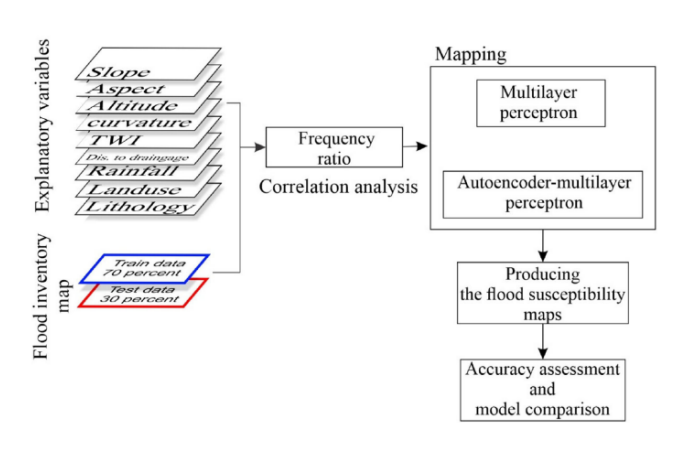
\includegraphics[width=1\textwidth]{Figures/AutoEncoder.png} % Adjust the width as needed
		\caption{Flowchart of the model proposed by\cite{ahmadlou2020}}
		\label{fig:my_label8} % Use this label to reference the figure elsewhere
	\end{figure}

	The study employed a hybrid model that combines a \ac{MLP} and an Autoencoder. 
	The data comprised geospatial features such as slope, curvature, aspect, altitude, rainfall, and 
	land use. Hidden representations of these features were derived using autoencoders.

	The dataset was categorized into five classes representing flood risk levels: very low, low, moderate, high, and very high. Given the labeled nature of this dataset, 
	they opted to use an \ac{MLP}, which is a supervised learning method, to determine the model weights.

	A \ac{MLP} is a type of neural network that consists of one input layer which in the case study consist
	of the hidden representations learned from the autoencoder, one or multiple hidden layers connected to a 
	output layer that predicts the class labels using the backpropogation algorithm along with a optimization
	algorithm like gradient descent to adjust model weight iteratively.

	\chapter{Data}
	\label{chap:methodology}

	For the task at hand, a novel methodology is proposed in this project. The features considered for this task, 
	can be subdivided into three classes:

	\begin{enumerate}
		\item \textbf{Terrain Information:} In this case, the elevation model, denoted by \ac{DEM}, was readily available from the \ac{SRTM} mission undertaken by \ac{USGS}. This data, with a spatial resolution of 30m, is superior to the data used in previous studies by other authors. Additionally, the slope of the terrain is another crucial factor. The slope determines the amount of solar irradiance incident on the surface of the \ac{PV} cells. Furthermore, a steep slope would not be suitable for a solar \ac{PV} farm.
		
		\item \textbf{Solar Irradiance and Atmospheric Conditions:} These were sourced from \ac{NREL}. They play a pivotal role in identifying suitable locations. Specifically, a region with high solar irradiance, minimal overcast conditions, and high temperatures would be ideal.
		
		\item \textbf{Other Features:} For this project, we also considered \ac{GIS} layers from the \ac{OSM} dataset. This includes features such as railways, roadways, land use, landmarks, and urban areas.
	\end{enumerate}
	
	The primary objective here is to employ K-means clustering to create clusters and identify the most suitable ones based on locations that already contain a solar PV plant within the appropriate cluster. 
	However, given the data's diversity and high dimensionality, it's essential to reduce its dimensionality and integrate our data from various sources before applying the clustering techniques.

	\section{Data Sources and Overview}

	For this project, we required multiple layers of GIS data that would serve as essential features for identifying suitable locations for solar farms. 
	Terrain information is a pivotal feature for this study. To set up a solar farm, vast expanses of land with minimal elevation changes are necessary. 
	Another critical attribute is solar irradiance, which is defined as the power potential generated from solar radiation incident on a specific location, 
	measured in watts per square meter (W/m\textsuperscript{2}). Additional crucial factors to consider include land cost, population density, land use, and 
	protected wildlife sanctuaries.

	

	\subsection{Terrain Data}

	The \ac{USGS}) is an agency of the United States government that operates across disciplines such as geology, geography, and hydrology. 
	The \ac{SRTM} was undertaken in collaboration with \ac{NASA} to create \ac{DEM} 
	of the earth's surface. This effort produced two Digital Elevation Models available for research, with spatial resolutions of 1 arc-second (30 meters) and 3 arc-second 
	(90 meters). For this study, we will be using the DEM model with a 1 arc-second spatial resolution\cite{farr2000}.

	\begin{figure}[H]
		\centering
		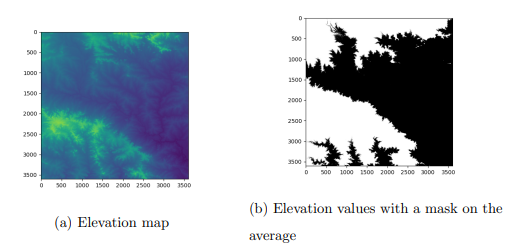
\includegraphics[width=0.8\textwidth]{Figures/Terrain.png} % Adjust the width as needed
		\caption{Elevation map for coordinates N 20' E 78}
		\label{fig:my_label2} % Use this label to reference the figure elsewhere
	\end{figure}

	\subsection{ Solar Irradiance Data}

	The \ac{NSRDB} provides a comprehensive collection of solar irradiance data. This database, which is calculated on both hourly and 
	half-hourly bases, is maintained by the \ac{NREL}, the U.S. Department of Energy, and various other contributors\cite{sengupta2018}. 

	Solar irradiance is characterized by three distinct measurements:

	\begin{itemize}
		\item \textbf{\ac{GHI}:} This refers to the total amount of solar radiation received per unit area on the Earth's surface. It is a cumulative measure that encompasses diffuse horizontal irradiance, ground-reflected radiation, and diffuse sky radiation.
		
		\item \textbf{\ac{DNI}:} \ac{DNI} indicates the amount of solar radiation received per unit area on a surface that is perpendicular to the sun rays incident on that surface.
		
		\item \textbf{\ac{DHI}:} This measurement pertains to the solar radiation that is scattered from the sky, excluding the direct solar beam.
	\end{itemize}

	\begin{figure}[H]
		\centering
		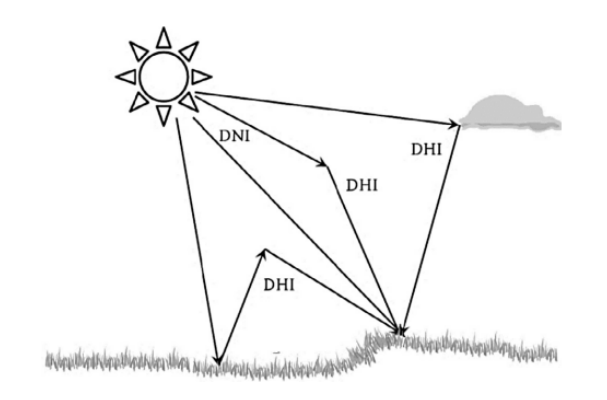
\includegraphics[width=0.5\textwidth]{Figures/Solar Irradiance.png} % Adjust the width as needed
		\caption{Solar Irradiance components\cite{vignola2023}}
		\label{fig:my_label3} % Use this label to reference the figure elsewhere
	\end{figure}


	\begin{figure}[H]
		\centering
		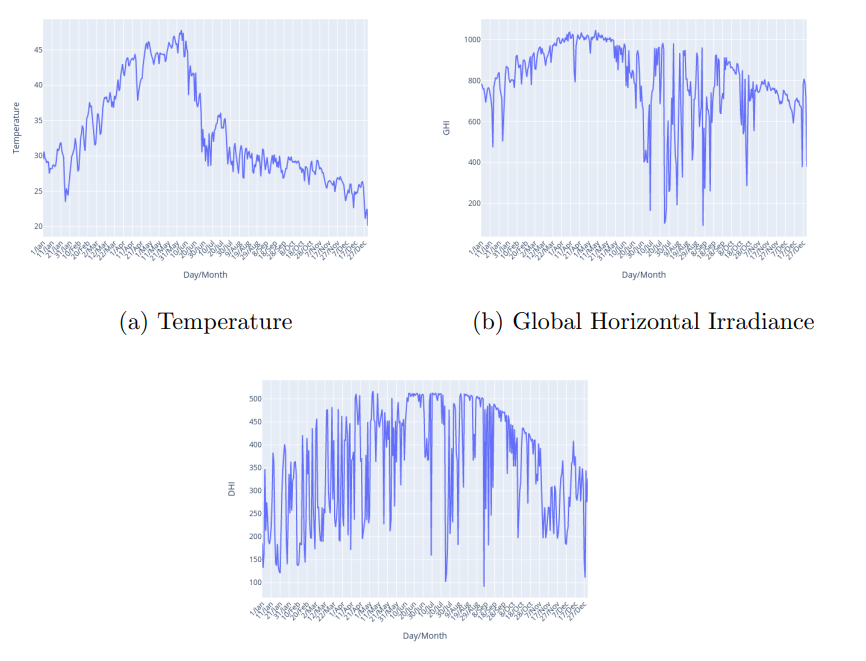
\includegraphics[width=1\textwidth]{Figures/Solar Graphs.png} % Adjust the width as needed
		\caption{Solar irradiance data for co-ordinates for coordinates N 20' E 78'}
		\label{fig:my_label4} % Use this label to reference the figure elsewhere
	\end{figure}

	\subsection{Other Important Attributes}

	While solar irradiance and elevation are critical features to consider when planning the setup of a solar farm, there are numerous other factors that warrant attention. 
	These include:

	\begin{itemize}
		\item \textbf{Financial Viability:} It's essential to assess whether there's sufficient demand for energy in the region to sustain a solar farm.
		
		\item \textbf{Environmental Impact:} Careful consideration must be given to the potential environmental repercussions of developing a solar plant, especially in ecologically sensitive regions.
		
		\item \textbf{Land-use Guidelines:} The designated or allowable uses of a land parcel can influence its suitability for solar farming.
		
		\item \textbf{Skilled Labor:} The availability of trained professionals and workers in the vicinity can have a bearing on the feasibility of the project.
	\end{itemize}

	\ac{OSM} is an open-source collaborative project initiated in 2004, with the objective of creating free geographic data. Over the years, 
	it has evolved into a global community-driven initiative. The maps and data generated by OSM collaborators can be leveraged for various attributes required 
	for such projects~\cite{openstreetmap2017}.
	\begin{figure}[H]
		\centering
		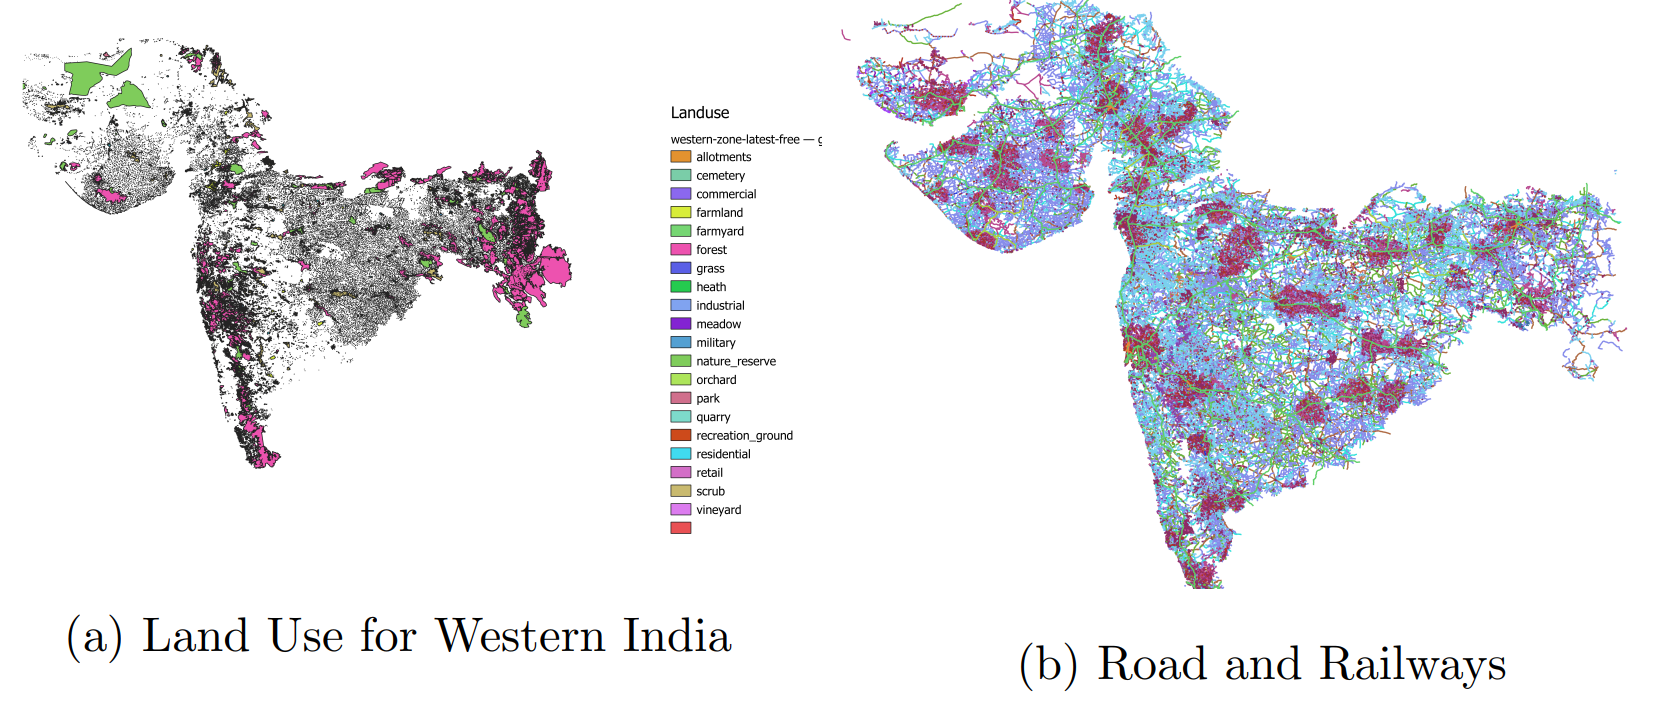
\includegraphics[width=1\textwidth]{Figures/Other attributes.png} % Adjust the width as needed
		\caption{Attributes for Western India}
		\label{fig:my_label5} % Use this label to reference the figure elsewhere
	\end{figure}


	\section{Data Modelling and Preprocessing}

	\subsection{Terrain Data}
		The terrain data, available as a \ac{DEM} model, boasts a spatial resolution of 30m and dimensions of \(3601 \times 3601\). Each matrix value in this model 
		represents the elevation. Consequently, each terrain data file encompasses an area of approximately 389,016 square kilometers. Although \ac{NREL} does not provide 
		direct slope data, it is possible to derive slope values from the elevation file. Mathematically, slope represents the rate of change of variable values. 
		Given that we possess the adjacent elevation values and that there's a consistent 30-meter distance between these values, a function can be formulated to determine the 
		slope values corresponding to the \ac{DEM} data file.

		Algorithm below showcases the calculation of slope matrix from the given elevation matrix.

		\begin{algorithm}[H]
			\caption{Calculate Slope from Elevation matrix}
			\begin{algorithmic}[1]
			\REQUIRE $matrix$, $spatial\_resolution$
			\ENSURE $slope\_matrix$
			\STATE $rows, cols \leftarrow \text{shape}(matrix)$
			\STATE $slope\_matrix \leftarrow \text{zeros matrix of size } (rows, cols)$
			\FOR{$i = 1$ to $rows-2$}
				\FOR{$j = 1$ to $cols-2$}
					\STATE $delta\_x \leftarrow matrix[i, j+1] - matrix[i, j-1]$
					\STATE $delta\_y \leftarrow matrix[i+1, j] - matrix[i-1, j]$
					\STATE $distance\_x \leftarrow 2 \times spatial\_resolution$
					\STATE $distance\_y \leftarrow 2 \times spatial\_resolution$
					\STATE $slope\_x \leftarrow \frac{delta\_x}{distance\_x}$
					\STATE $slope\_y \leftarrow \frac{delta\_y}{distance\_y}$
					\STATE $slope \leftarrow \sqrt{slope\_x^2 + slope\_y^2}$
					\STATE $slope\_matrix[i, j] \leftarrow slope$
				\ENDFOR
			\ENDFOR
			\RETURN $slope\_matrix$
			\end{algorithmic}
		\end{algorithm}

		By following the algorithm, one can obtain a matrix that provides an approximation of the slope at each cell in the DEM.

		

	\subsection{Solar Irradiance and Atmospheric Conditions Data}

	The atmospheric conditions data, fetched from \ac{NREL}, is presented in the form of a time series for specific locations. For the model, 
	we utilize the mean of the time series of various attributes (GHI, DHI, DNI, Clearsky DHI, Clearsky DNI, Clearsky GHI, Temperature, Relative Humidity). 
	Essentially, we compute the mean of the time series for each location for which we have both elevation and slope data available.


	\subsection{Other \ac{GIS} features}
	
	The \ac{GIS} encompasses features such as railways, roadways, land use, landmarks, and urban areas. These features are represented as shapefiles, which comprise polygons 
	mapped onto a coordinate system. These polygons facilitate the assignment of specific characteristics to designated areas. After utilizing the terrain data and atmospheric 
	condition attributes for clustering, we will leverage the \ac{GIS} features to develop a rule-based classifier. This classifier aims to subset land based on the polygon values 
	from the \ac{GIS} layers, as detailed in the associated table.

	{\scriptsize
	\begin{longtable}{|p{2cm}|p{12cm}|p{2cm}|}
		\caption{Spatial Data Classification} \\
		\hline
		\textbf{Category} & \textbf{Occupied space for a purpose, cannot be used for solar pv plants} & \textbf{Unoccupied/ Vacant can be used} \\
		\hline
		\endfirsthead
		\multicolumn{3}{c}%
		{{\bfseries \tablename\ \thetable{} -- continued from previous page}} \\
		\hline 
		\textbf{Category} & \textbf{Occupied space for a purpose} & \textbf{Unoccupied/ Vacant can be used} \\
		\hline 
		\endhead
		
		\hline \multicolumn{3}{|r|}{{Continued on next page}} \\ \hline
		\endfoot
		
		\hline
		\endlastfoot
		
		Buildings & place\_of\_worship, parking, hotel, apartments, commercial, tower, train\_station, hospital, house, university, dormitory, school, college, residential, industrial, bungalow, civic, attraction, transportation, storage\_tank, cinema, stadium, service, depot, church, building, temple, fire\_station, library, bank, public, retail, ruins, office, police, terrace, canteen, cafe, collapsed, mosque, restaurant, bus\_station, memorial, construction, public\_building, sports\_centre, hostel, garage, supermarket, roof, toilets, hut, central\_office, apartment, mall, wall, theatre, shed, detached, courthouse, clinic, workshop, fuel, cabin, post\_office, marketplace, childcare, warehouse, community\_centre, water\_tower, fast\_food, manufacture, blood\_bank, events\_venue, townhall, part, prep\_school, guest\_house, social\_facility, gallery, arts\_centre, kindergarten, yes,\_hotel,\_comm, hangar, yes, bar, ferry\_terminal, greenhouse, fort, chapel, works, factory, shop, shelter, stage, city\_gate, tomb, veterinary, lighthouse, car\_wash, pumping\_station, outdoor, motorcycle\_parki, social\_centre, clubhouse, motel, substation, food\_court, stupa, government, pier, cowshed, aquarium, pharmacy & undefined, nan, vacant \\
		\hline
		landuse & commercial, retail, residential, recreation\_groun, railway, salt\_pond, grass, industrial, military, cemetery, plant\_nursery, farmland, construction, basin, garages, quarry, reservoir, saltpond, brownfield, landfill, religious, allotments, yes, green, orchard, garden, village\_green, education, farmyard, aquaculture, parking, used by school a & barren, meadow, vacant, greenfield \\
		\hline
		places & city, neighbourhood, locality, suburb, hamlet, village, town, island, yes, farm, plot, borough & None \\
		\hline
		railway & rail, platform, subway, miniature, monorail, construction, platform\_edge, traverser, workshop, turntable, proposed & abandoned, disused \\
		\hline
		natural & water, forest, park & - \\
		\hline
		waterways & drain, river, stream, dam, weir, canal, dock & unclassified \\
		\hline
		road & residential, motorway, tertiary, service, trunk, path, secondary, primary, living\_street, construction, footway, primary\_link, track, motorway\_link, trunk\_link, steps, pedestrian, secondary\_link, tertiary\_link, bridleway, proposed, cycleway, elevator, bus\_stop, services & - \\
		\hline
		points & switch, station, level\_crossing, stop, traffic\_signals, hotel, clinic, crossing, school, parking, mini\_roundabout, bus\_stop, hospital, restaurant, place\_of\_worship, motorway\_junctio, attraction, ruins, studio, bank, theatre, fast\_food, ice\_cream, college, pharmacy, cafe, police, The Wall, pub, toilets, memorial, fuel, telephone, ferry\_terminal, buffer\_stop, water\_tower, hostel, post\_box, bus\_station, lighthouse, atm, theme\_park, fire\_station, community\_centre, post\_office, fountain, picnic\_site, works, cinema, marketplace, bar, monument, kindergarten, signal, railway\_crossing, car\_wash, doctors, townhall, viewpoint, clubhouse, guest\_house, drinking\_water, museum, battlefield, library, taxi, turning\_circle, artwork, water\_well, motel, fort, childcare, social\_centre, tower, surveillance, flagpole, dentist, rest\_area, vending\_machine, public, passing\_place, spa, parking\_entrance, unclassified, bureau\_de\_change, platform, information, nightclub, chimney, bench, turning\_loop, car\_rental, internet\_cafe, camp\_site, events\_venue, veterinary, gallery, crematorium, wayside\_cross, waste\_basket, stage, city\_gate, garage, taxi\_rank, arts\_centre, hairdresser, border\_control, swimming\_pool, water\_mill, milestone, well, fishing, bbq, leisure, lodge, boat\_rental, water\_tap, embassy, laundry, razor, bollard, power, toll\_gate, street\_lamp, photo\_booth, pitch, water\_point, barrier, prison, convenience, park, speed\_camera, graveyard, bench & unclassified \\
		\hline
		\end{longtable}}


		In the table above, the 'Category' represents the layers of \ac{GIS}, while the other columns contain the values associated with those layers. These values specify the type of location, represented as polygons, for the corresponding \ac{GIS} layer.


	\begin{figure}[H]
		\centering
		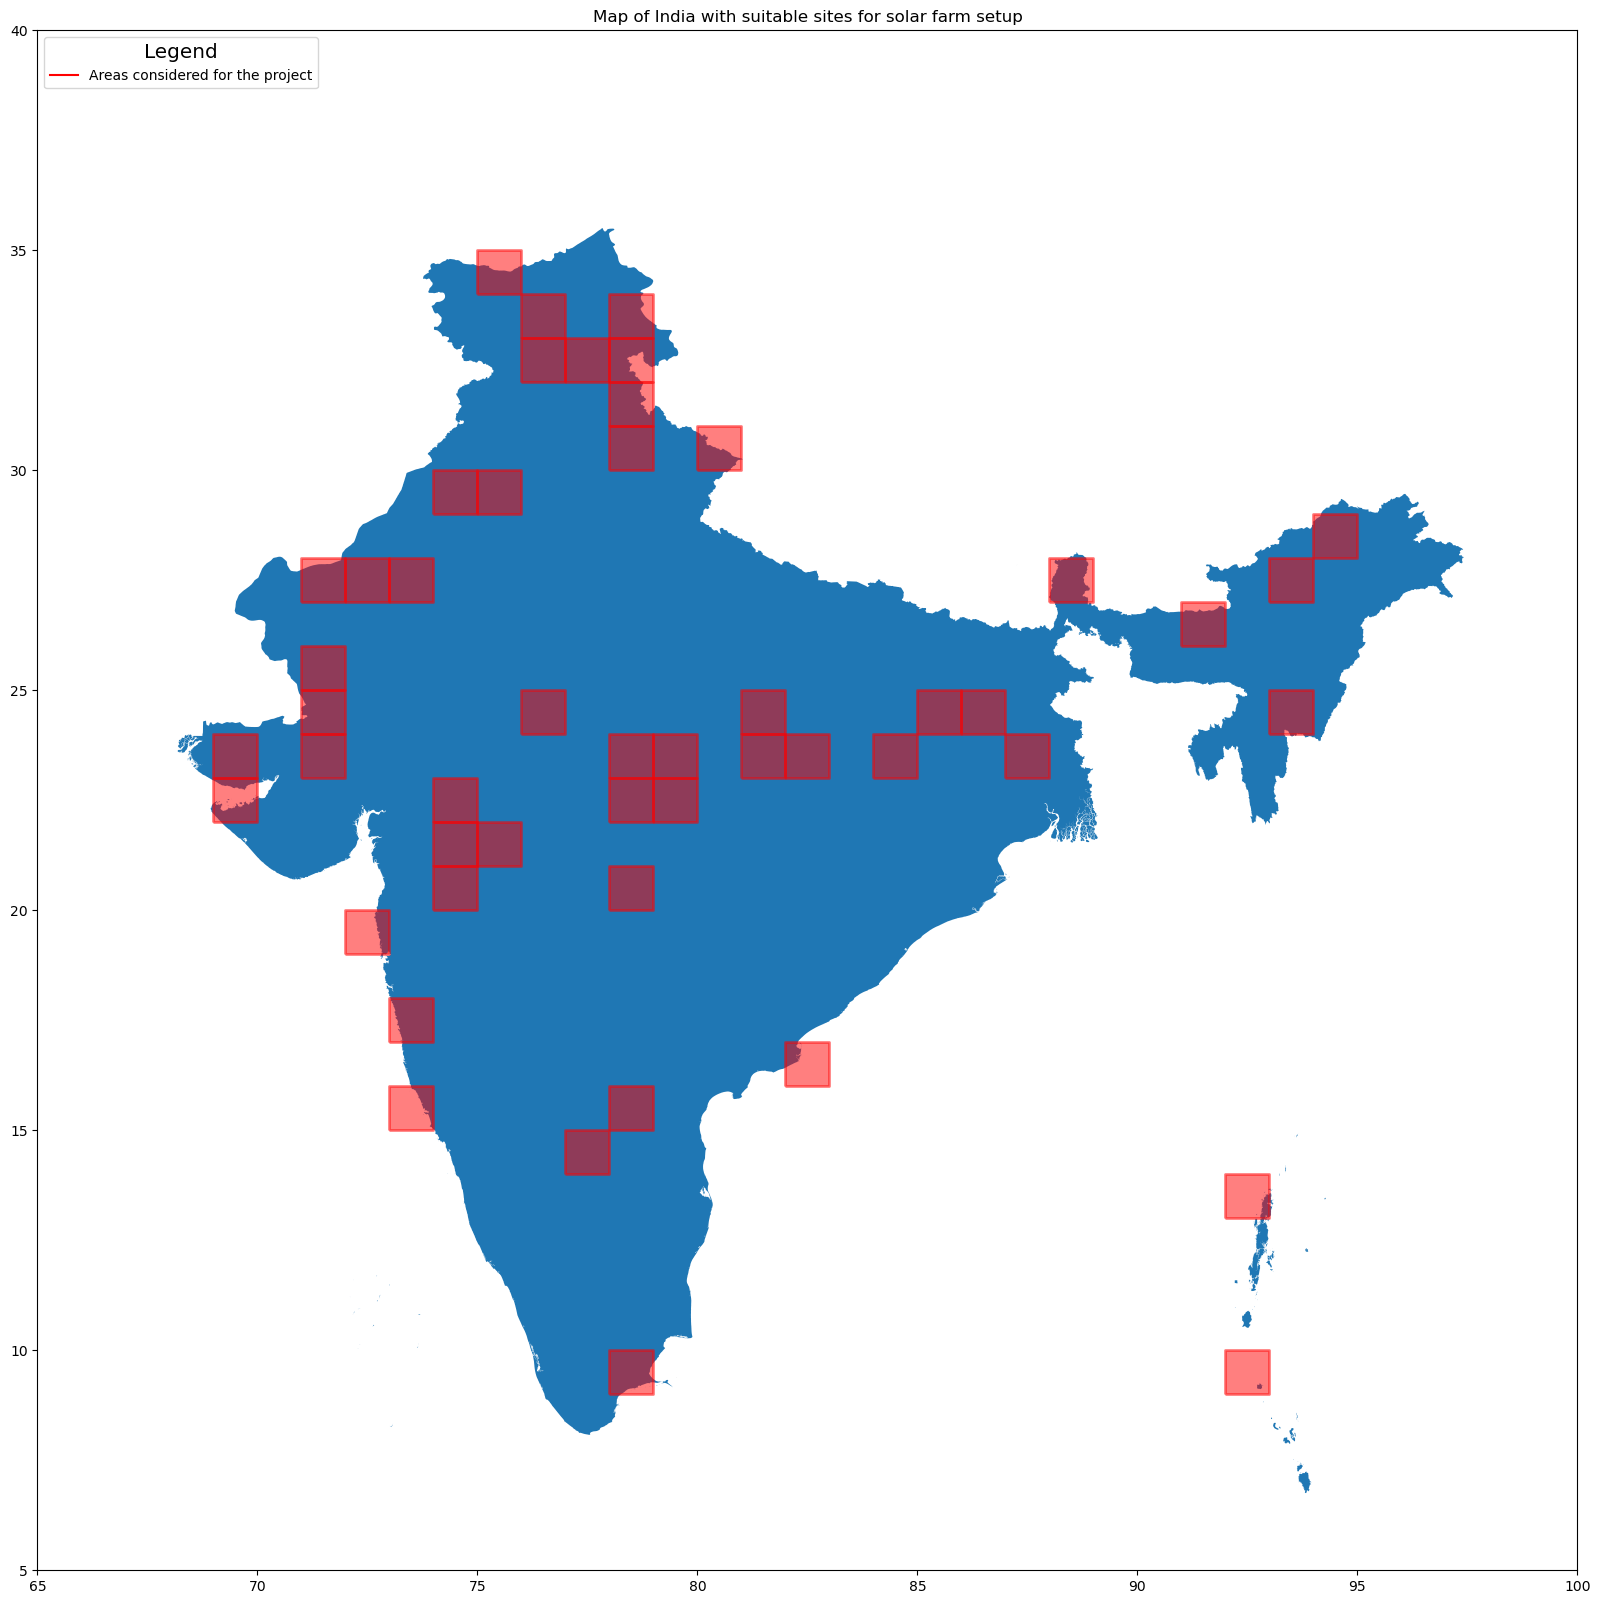
\includegraphics[width=0.8\textwidth]{Figures/india_map_with_highlighted_data.png} % Adjust the width as needed
		\caption{Map with areas highlighted that are considered for the study containing the Elevation and Slope data, solar irradiance and atmospheric conditions data and GIS information}
		\label{fig:my_label9} % Use this label to reference the figure elsewhere
	\end{figure}


	Figure \ref{fig:my_label9} highlights the geographic areas considered for this study. These specific 
	regions were selected to capture a diverse range of locations for representation in the autoencoder. 
	The chosen regions encompass a variety of geographical features, including tall mountains, desert 
	landscapes, plains, plateaus, and islands.


	\subsection{Limitations of dataset}

	The data regarding slope and elevation features boasts impressive quality, with a spatial resolution of 30m. However, there's a gap in our matrix when it comes
	 to atmospheric conditions. Instead of comprehensive coverage, this data is available solely as a time series for specific locations. Additionally, due to time and 
	 resource constraints, we only have 50 data samples to test the model. This limited dataset might 
	 present challenges in obtaining a holistic understanding, and as we move forward, it's imperative 
	 to optimally use this limited set for accurate model testing.
	 
	\chapter{Methodology}

	\section{Overview}

	Autoencoders, as a neural network architecture, have been an essential subject of research in deep learning. 
	A foundational understanding of autoencoders can be traced back to the works of Rumelhart et al. and 
	Hinton et al \cite{rumelhart1986} \cite{Hinton2006}. As presented in Chapter 2, these studies laid the groundwork for the current application and 
	understanding of autoencoders. The Deep Autoencoder, emerging from these foundational studies, serves as the primary focus of this investigation.

	\section{AutoEncoder}

	\subsection{Introduction}

	Data prepared from steps for Data Preprocessing and Modelling that were discussed in Chapter 3 would be
	used for developing the Autoencoder for this study. The Elevation data matrix, Slope data matric that was created 
	using Algorithm 1, Atmospheric condition features include \ac{GHI}, \ac{DHI}, \ac{DNI}, Clearsky\_GHI, Clearsky\_DHI, 
	Clearsky\_DNI, Temperature, Relative Humidity. 

	Initially, given that the data for Slope and Elevation are represented as matrices, they are to be processed using two 
	deep autoencoders with similar architectures. This is done after normalizing these matrices. Once these intermediate 
	representations or embeddings are generated, they will be concatenated and passed to another autoencoder. This process 
	aims to yield the final embeddings, which will be utilized for clustering regions with similar geographical 
	features. Since the data for solar irradiance and atmospheric conditions are singular values, they will be fed into the 
	final autoencoder. This will be done after dimensionality reduction of the concatenated embeddings through a few initial layers.


	\subsection{Model Architecture}

	The data for dual deep autoencoders for the slope and elevation matrices are in from of matrixes with each
	value in matrix represention the elevation in meters and the slope gradient value at a spatial resolution of 
	30 meters. 

	Since the data is in the form of two-dimensional matrices, they can be fed through initial layers of convolutional 
	layers for feature extraction. 
	
	Terminologies used in \ac{CNNs}
	\begin{itemize}
		\item \textbf{Convolution Operation: }At its core, convolution operations involve taking a filter of a size smaller than the 
		input and slides it over the input to produce a feature maps.During the training phase of a \ac{CNN}, after the forward pass on the network the error is backpropogated
		and the filter/kernel values are adjusted based on partial derivatives of previous errors. 
		\item \textbf{Kernel/Filters: }The kernels slide over the input matrix to produce the feature map. The number of kernels determine the amount of feature maps
		that can be produces. The dimensions of the kernels should match the image dimension for it to convolve over the matrix.
		\item \textbf{Stride: } The value of stride determines the movement of filter over the input matrix. A stride value of 1
		moves one pixel right at a time, for the value 2 it moves 2 pixels at the time. the value of stride determine the output matrix dimensions.
		\item \textbf{Padding: }Padding involves adding a vector border of zeroes around the input to control the spatial size of 
		output matrix and to ensure that the border pixels of the input matrix are processed with equal weightage.
	 \end{itemize}

	 To gee the size of the output matrix after convolution operations we can you the below formula, where
	 $\textit{W}_{in}$ the width of input matrix, \textit{F} is the filter size and \textit{S} is the stride value and
	 $\textit{W}_{out}$ is the dimension of output matrix

	 \[W_{\text{out}} = \left\lfloor \frac{W_{\text{in}} - F + 2P}{S} + 1 \right\rfloor\]

	 In the autoencoder architecture, the encoder is responsible for generating embeddings through the application of convolution 
	 layers followed by dense layers. Consequently, the decoder seeks to upscale these embeddings. When considering the dense linear 
	 layers within the decoder, it is necessary to mirror the architecture of the dense layers present in the encoder. To recreate the 
	 spatial feature maps before they undergo the convolution process, the transposed convolution operation is used to learn the filters 
	 for deconvolutional layers in the decoder.

	 The transposed convolution formula to upscale the feature maps in decoder where $\textit{W}_{in}$ the width of input matrix, \textit{F} is the filter size and \textit{S} is the stride value and
	 $\textit{W}_{out}$ is the dimension of output matrix

	 \[W_{\text{out}} = (W_{\text{in}} - 1) \times S - 2P + (F - 1) + 1\]

	


	\section{Clustering}

	With the embeddings created through thhe final autoencoder, K-means clustering an unsupervised 
	clustering technique will be used to get cluster similar geospatial regions based on their euclidean distance 
	and proximity to a centroid.

	K-means clustering is a popular clustering technique that is widely recognised for its simiplicity, computational 
	efficiency, interpretablity.

	The \textit{K} in K-means represents the number of clusters to be considered for the data in the latent space of the 
	autoencoder. Initially, the centroids are randomly selected within this latent space. Consequently, each datapoint in 
	the latent space is assigned to a cluster based on its proximity to the centroids. This proximity is measured using 
	distance metrics such as Euclidean, Manhattan, and Minkowski distances. After assignment, the centroids are recalculated 
	based on the data points assigned to them in the previous step. The process continues iteratively until convergence. Here,
	 \textit{"convergence"} typically signifies that the centroids remain relatively stable, with no significant shifts in their 
	 positions compared to earlier iterations.

	 The popularity of K-means doesn't overshadow its shortcomings. In unsupervised learning problems, the value of \textit{K} 
	 is typically unknown. The Elbow curve method is one technique employed to determine the appropriate value for \textit{K}. 
	 Iteratively, different values for \textit{K}, usually ranging from 1 to 10, are used to generate multiple K-means models. 
	 For each model, the sum-of-squared distances from the points to their respective centroids are computed. These values are 
	 then plotted against the corresponding \textit{K} values. The \textit{Elbow} point on this curve is where the rate of decrease 
	 in the sum-of-squared distances sharply changes. Although this point is often considered a good estimate for \textit{K}, it doesn't 
	 guarantee an optimal number of clusters. Another significant concern with K-means clustering is the algorithm's potential to get stuck in a local minimum.


	\section{Rule-Based Classifier}

	After clustering, we can analyze the results to identify suitable locations by looking for locations that have pre-existing solar PV plants, considering the 
	geographic features of the datapoints in each cluster, etc. 

	After subsetting the data points based on the cluster, we can select the geospatial locations that correspond to the embeddings of those data points. These 
	geospatial locations were chosen based on several factors including terrain features, slope, elevation, and atmospheric conditions such as solar irradiance, 
	humidity, and temperature. However, even with these considerations, there is still a lack of clarity regarding which regions are suitable for solar PV plants. 
	This is because we have not taken into account \ac{GIS} layer information such as urban and rural centers, roadways, railways, and land use of the area. We will utilize 
	the \ac{GIS} information we have collected for these regions to further refine our selection.

	The \ac{GIS} data for the geospatial locations is available for 8 categories, for each category there are various
	attributes with their corresponding area polygons which can be considered suitable or unsuitable for this study.

	For example, for the layer landuse the attributes barren, vacant and greenfield can be suitable, but attributes city,
	neighbourhood, suburb cannot will be unsuitanble for our purpose. Based on above arguments we can make a rule 
	based classifier that crops land that would be suitable for solar PV plant installation for the geospatial locations
	selected through the process of clustering. 
	
	\begin{itemize}
		\item \textbf{Buildings: } This layer contains attributes associated with human development and therefore most of the attributes would contain area polygons that would be unsuitable with few expections 
		like attributes vacant and None in the dataset.
		\item \textbf{Landuse: } This layer contains attributes related to the type of activity the land is accredited to. Attributes such as barren, vacant, greenfield could be particularly useful for this study.
		\item \textbf{Places: } Collection of human settlements like city, locality, industrial are contained in this layer.
		\item \textbf{Railways, Roads and waterways : } Transit systems are defined in this layer as area polygons around the roads and railways.
		\item \textbf{Natural: } Nature and wildlife reserves along with water bodies are highlighed in this layer.
		\item \textbf{Points: } Any human developed structure like guest houses, water towers, rest areas are highlighted in this region.
	\end{itemize}

	The whole list of the attributes that are suitable and unsuitable are given in table 3.1

	
	\chapter{Experiments}

	\section{Experiments}
	\section{Results}

	\chapter{Conclusion}
	\label{chap:conclusion}
	\section{Limitations}
	\section{Conclusion}

	
	Here you must zoom back out to evaluate the thesis. Mention limitations and weaknesses as well as contributions and possible future work.
	
	%%%%%%%%%%%%%%%%%%%%%%%%%%%%%%%%%%%%%%%%%%%%%%%%%%%%%%%%%%%%%%%%%%%%%%%%%%%%%%%%
	%\bibliographystyle{plainnat}                  % to give author-year style
	\bibliographystyle{IEEEtranN} 
	\renewcommand{\bibname}{References}           % change default name Bibliography to References
	\bibliography{references}                     % BibTeX References file, references.bib
	\addcontentsline{toc}{chapter}{References}    % add References to TOC
	
	
	%%% uncomment if Appendix needed
	%\appendix
	%\chapter{Appendix-A-Title} 
	%\label{chap:appendix_a}
	
	%\chapter{Appendix-B-Title} 
	%\label{chap:appendix_b}
	
\end{document}
